\section{Visualizing Electromagnetic Plane Waves}

\instructornote{ 
By Jerry, Dec, 2020. Activity 3 of the lab had to be redone because the Java applets no longer work because of security changes. We substituted
the previous java applet with a java jar file that is less sophisticated, but adequate. See the unit for the address of the software.
}

\makelabheader %(Space for student name, etc., defined in master.tex)

\bigskip
\textbf{Objective:} 


To investigate electromagnetic waves, using two different software simulations.

%\begin{itemize}
%\item The effect of changing magnetic fields on induced emf and current.
%\end{itemize}

\bigskip

\textbf{Activity 1: Simulating $\vv{\textit{E}}$, $\vv{\textit{B}}$, and $\vv{\textit{S}}$ in Electromagnetic Waves}


Open \textit{Firefox} and go to the website
\verb!http://www.falstad.com/emwave2!. A Java applet will pop up showing
brightly colored waves like the ones in Figure 1 propagating outward. 
%from our oscillating electric dipole. 
If you don't see this window, consult your instructor.
\begin{figure}[hbt]
\begin{center}
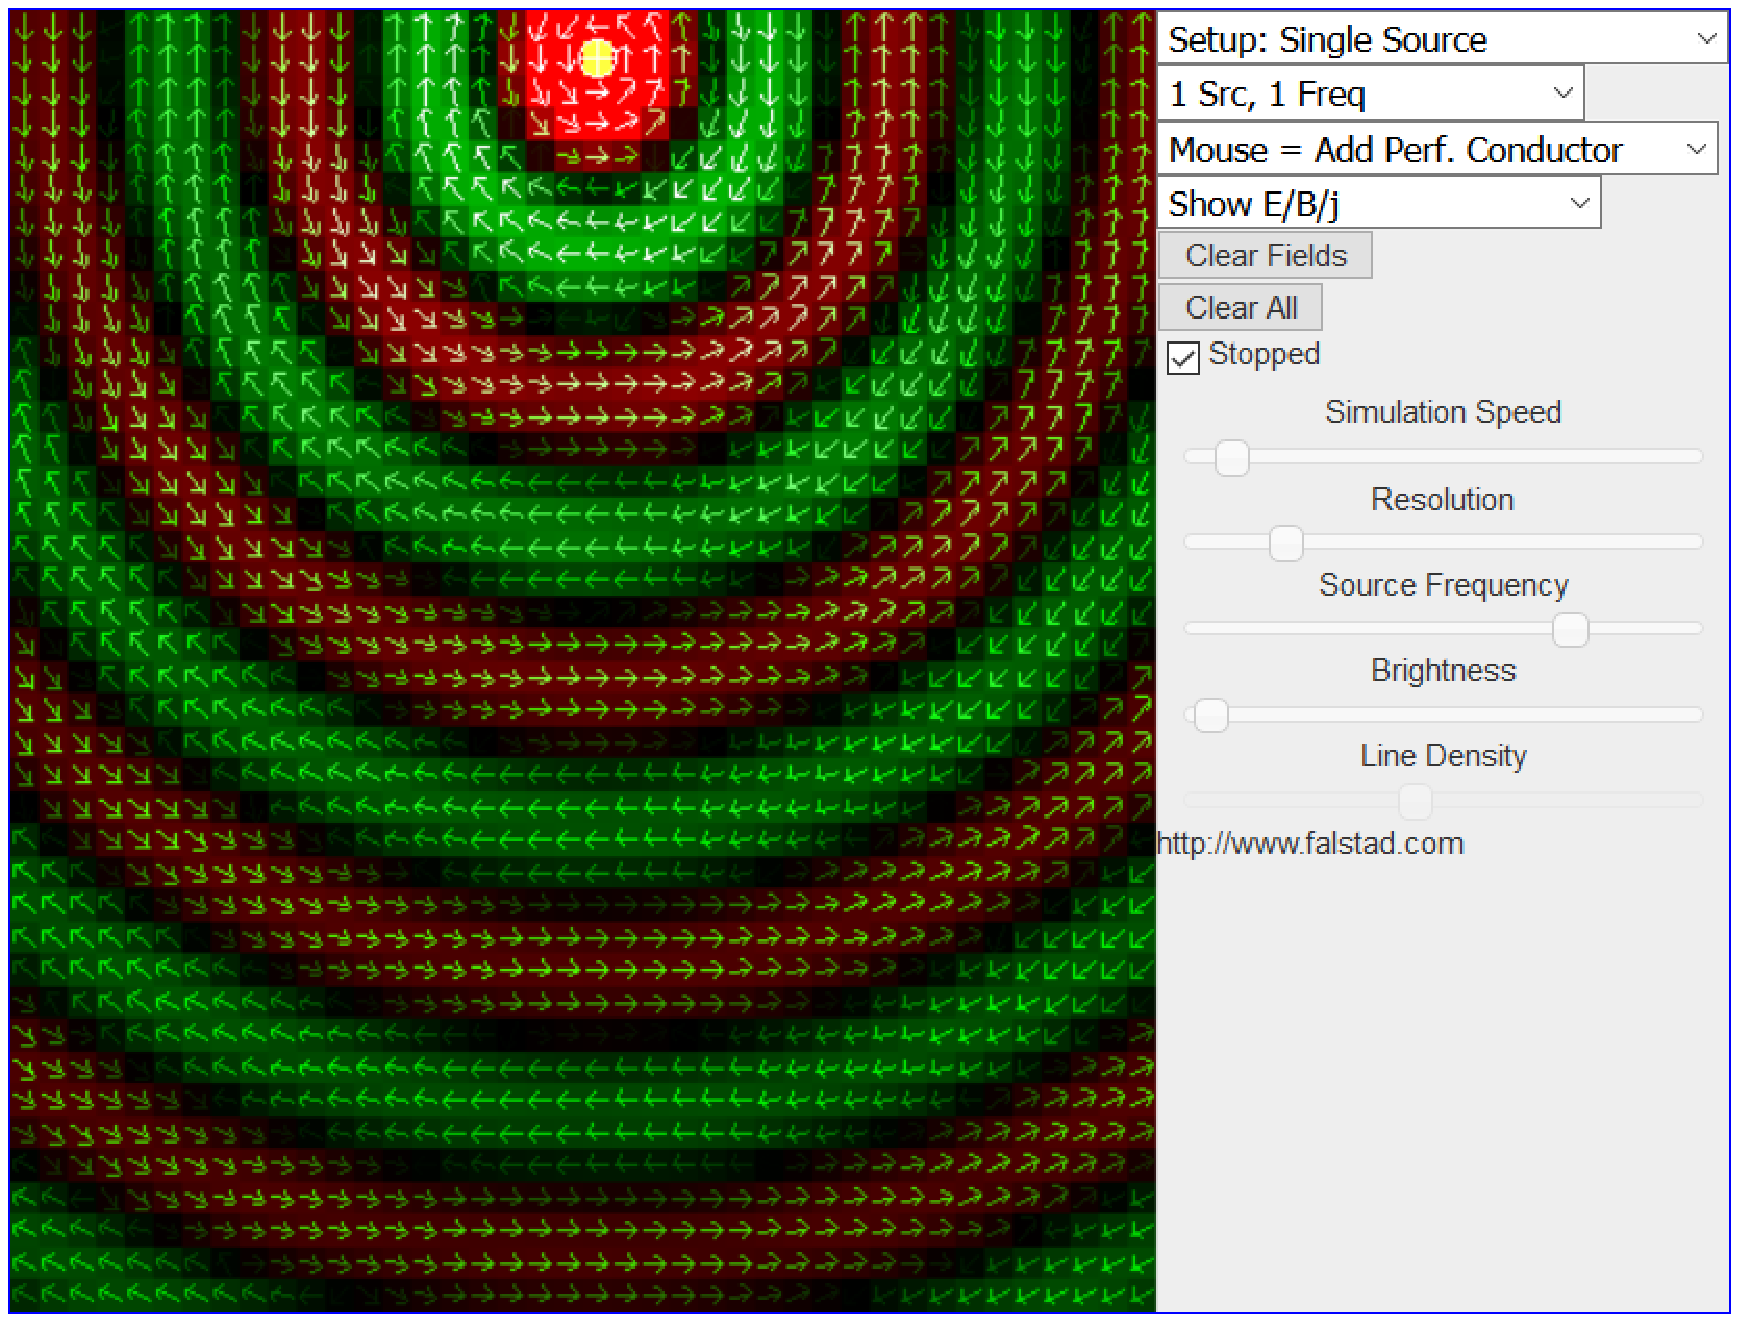
\includegraphics[width=6.0in]{plane_waves/falstad_screen.pdf}
\caption{Applet showing electromagnetic waves.}
\index{color page}
\end{center}
\end{figure}

\vspace{-0.2in}

It is useful to slow down the simulation speed to observe the waves more clearly.
Do this using the slide labeled
\texttt{Simulation Speed} on the right-hand side of the applet window.

\begin{enumerate}[labparts]

\item What you see is an ``oscillating dipole'', very similar to the generation of radio waves with an antenna.
Charges (usually electrons) are driven up and down in the antenna and emit electromagnetic 
waves.  
The alternating yellow and blue circle at the top of the applet is the source (the dipole)
as viewed from above.  Any yellow in the simulation indicates electrical current (charge) moving towards you, and any blue indicates current away from you.  Does the simulation show any current (motion of charges) flowing far away from the source?
\answerspace{1.0cm}

\pagebreak[2]
The green and red colors indicate the electric field; green areas are positive 
($\vv{E}$ toward you) and red areas are negative ($\vv{E}$ away from you). 
The electric field is always perpendicular to the plane of the screen.
In addition to the colors, arrows indicate the 
direction of the magnetic field, which is always in the plane of the screen.  

\item What direction does the electric field point when the magnetic field is to the right?
\answerspace{0.6cm}

\item What direction does the electric field point when the magnetic field is to the left?
\answerspace{0.6cm}

\item Are the electric and magnetic fields always perperndicular to each other?
\answerspace{0.6cm}

\item If you made predictions in Activity 2 of Lab \ref{induction_intro} about the directions of the $\vv {E}$ 
and $\vv {B}$ fields, compare those predictions with your observations here. Correct any disagreements.
\answerspace{2.0cm}

The ``Poynting vector'' $\vv{S}$ is defined to point in the direction of the flow of energy in a wave. Its direction is given by $\vv {E} \times \vv {B}$.  

\item What is the direction of $\vv {E}\times \vv {B}$ where the color of the wave is red?
\answerspace{1.0cm}

\item What is the direction of $\vv {E} \times \vv {B}$ where the color of the wave is green?
\answerspace{1.0cm}

\item Make the applet draw the Poynting vector by clicking on the arrow in the box with 
\texttt{Show E/B/j} entered in it. Scroll up or down until you find
\texttt{Show Poynting vector} and highlight it.
In what direction does the energy flow?  (Does that agree with what you just said about $\vv {E} \times \vv {B}$?)
\answerspace{1.0cm}

\end{enumerate}

\textbf{Activity 2: Wave Fronts, Wavelength, and Interference}


When you drop a pebble in a pond of water, the waves go out in circles. The shape of the ``wave front'', which is what you get when you connect all the points on the crest of a single wave, is a circle.   

\begin{enumerate}[labparts]

\item In this simulation, the waves are radiating out in three dimensions, not two.  In this three-dimensional case, what is the shape of the wave fronts?
\answerspace{1cm}

\item Far away from the pebble in the pond, the circular wave fronts hitting the shore look like straight lines because at a small length scale you don't notice their slight curvature. 
In the three-dimensional case in the simulation, what is the apparent shape of a wave front far away from the source, if you ignore the slight curvature?
\answerspace{1cm}


\pagebreak[2]

\item The distance between successive peaks or crests of the waves, shown by the green regions in the
applet, is called the wavelength.  
Light, for example, is an electromagnetic wave and different wavelengths correspond 
to different colors.
Reduce the frequency of the oscillation of the dipole using the slide labeled
\texttt{Source Frequency} on the right-hand side of the applet.
(You may have to increase the brightness of the applet using the slide labeled
\texttt{Brightness}.)
What happens to the wavelength when you decrease the frequency?
\answerspace{1.0cm}


\item Just for fun, we want to introduce one of the central phenomena associated
with waves known as interference.
Go back to the \texttt{Show E/B/j} mode you were in before. 
Go to the second menu from the top of the right-hand side of the applet, and select
\texttt{2 Src, 1 Freq}.
This will place an additional oscillating dipole at the bottom of the applet.  Use your mouse to drag the source from the bottom to the top right corner of the screen.

In the space below, make a rough sketch of what you see.  Label areas where waves from the two sources combine to cancel each other out (``destructive interference'') and areas where their amplitudes add (``constructive interference'').  If these were visible light waves, where would you see bright light?
\answerspace{40mm}
%\vfill

\end{enumerate}

\textbf{Activity 3: Plane Waves}

Open the file \filename{wave\_sim.cdf} in the \filename{\coursefolder} folder.  It should open in \button{Mathematica}.  You may need to click a button to ``Enable Dynamics,'' but then you should see a screen like the image below.

\begin{center}
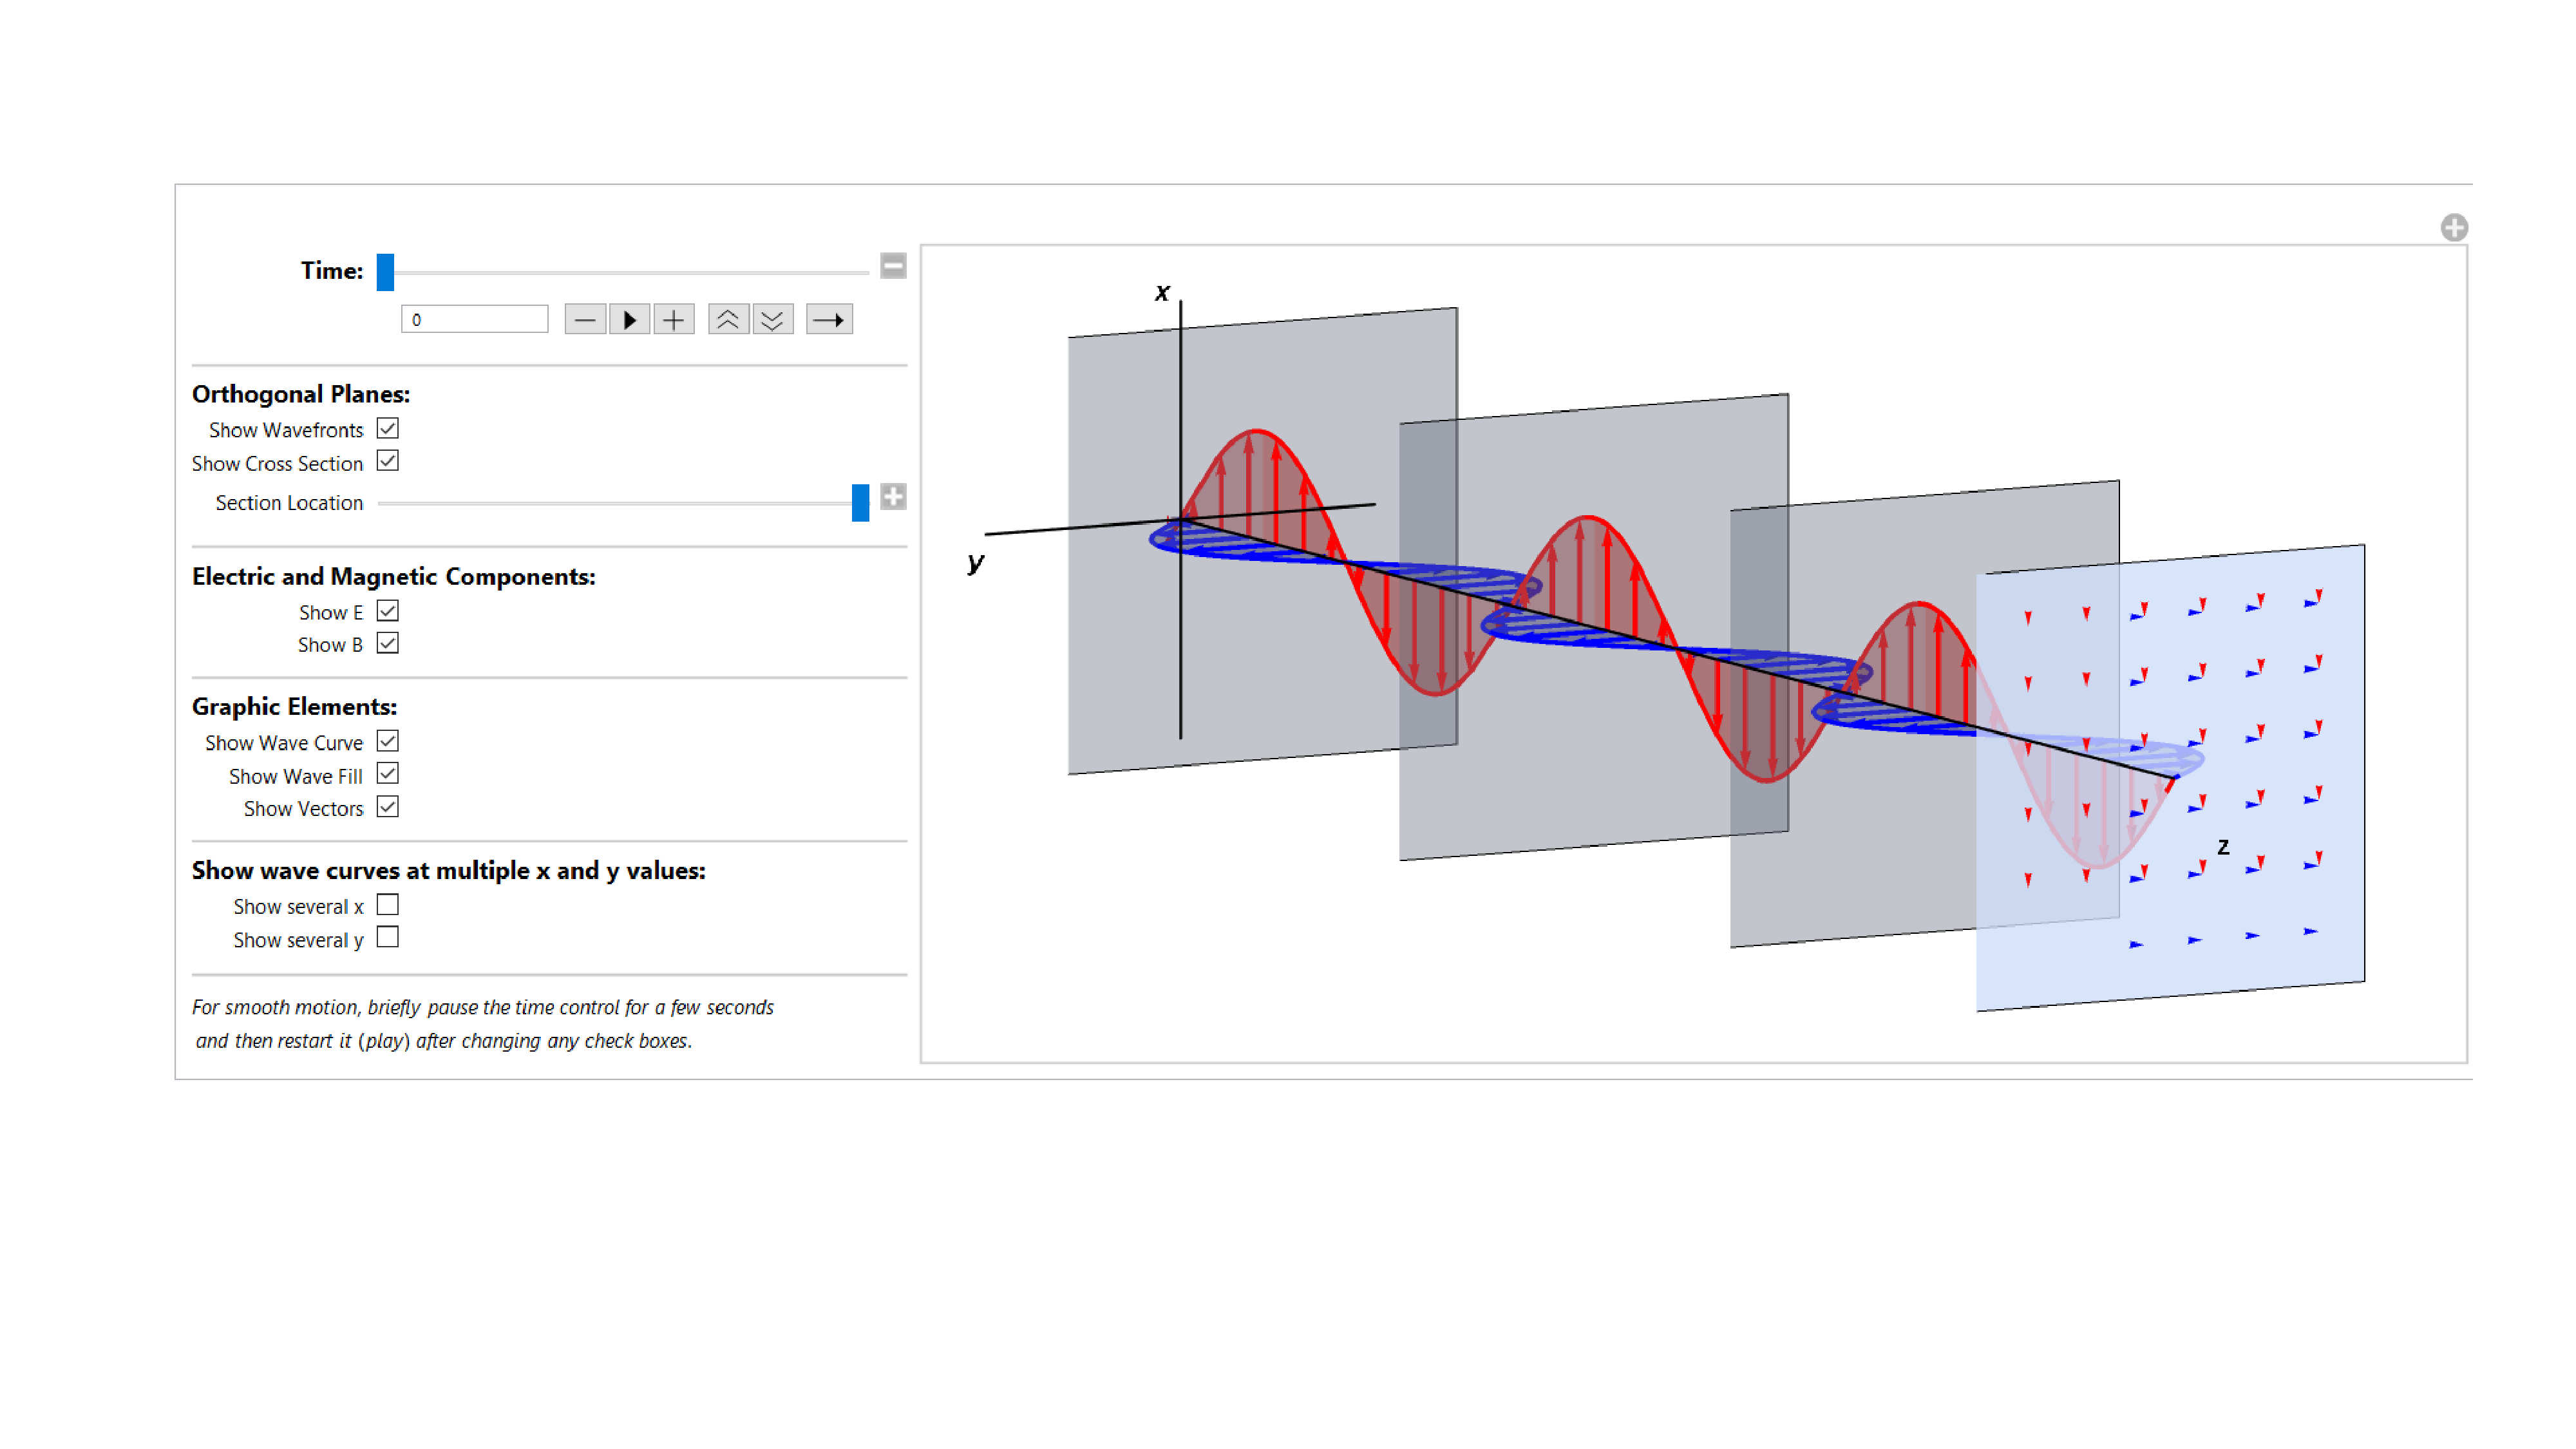
\includegraphics[width=\textwidth]{plane_waves/mathematica_applet/screen_shot.pdf}
\end{center}

To run the simulation, click on the trianglar play icon
(\raisebox{-0.7ex}{
\includegraphics[width=1.5em]{plane_waves/mathematica_applet/play_icon.pdf}})
\index{color_page}
in the \button{Time} control area.

\pagebreak[2]
\begin{enumerate}[labparts]
\item The simulation shows electric field and magnetic field vectors using two different colors.  Try unclicking the boxes labeled \button{Show E} and \button{Show B} to see which is which.  What is the orientation of the $\vv {E}$ field?
What is the orientation of the $\vv {B}$ field?
\answerspace{15mm}

(After messing with the check boxes, you may find that the motion of the simulation is slow and choppy.  To fix this, click the \button{pause} button, wait five seconds, and then hit \button{play} to restart it.)

\item Does $\vv {E} \times \vv {B}$ point in the direction of energy flow, 
as it did in the previous activity?
\answerspace{10mm}

\item The simulation shows several wavefronts which travel with the wave.  Do the wavefronts mark regions where the values of $\vv {E}$ and $\vv {B}$ are maxima, or where they are minima?
\answerspace{15mm}

\item The red and blue vectors representing $\vv {E}$ and $\vv {B}$ show the values of the fields along the $z$ axis, at $x=0$ and $y=0$.  To see the values of these fields at different $x$ and $y$ values, try clicking the boxes labeled \button{Show several $x$} and \button{Show several $y$}.  Does $\vv {E}=0$ away from the $z$ axis?  What about $\vv {B}$?
\answerspace{10mm}

\textit{Showing  $\vv {E}$ and $\vv {B}$ at all $x$ and $y$ is technically more accurate, but it makes a giant mess.  So we usually just draw them along one line (the $z$ axis here) to keep things tidy, even though $\vv {E}$ and $\vv {B}$ are really everywhere.}

\item Uncheck the \button{Show several $x$} and $y$ boxes, and uncheck \button{Show Wavefronts} too.  With the simulation paused, use the slider to move the cross-section plane back and forth along the $z$ axis.  The small red and blue arrows in the plane show the direction of the $\vv {E}$ and $\vv {B}$ fields at each point in $x$ and $y$.  Do the fields vary in $x$ and $y$, or are they \textit{uniform}?
\answerspace{10mm}

\item In general, electric and magnetic fields can be functions of $x$, $y$, $z$, and time $t$. However, for a plane wave traveling in the $+z$ direction, $\vv {E}$ and $\vv {B}$ only depend on two of those four variables.  Which ones?
\answerspace{10mm}

\item The electromagnetic wave in this simulation is shown by three different graphical elements: the solid red and blue wavy lines, the translucent filled areas below those wavy lines, and the $\vv {E}$ and $\vv {B}$ vectors regularly spaced along the $z$ axis.  (You can play with checking and unchecking them if you like.)  Do any these three representations convey specific information not in the others, or are these elements redundant?
\answerspace{10mm}
 

\end{enumerate}

\begin{comment}
% This commented-out part uses a different simulation.  I believe Jerry put this together from
% an online source in about 2020.
Go to this site to download a simulation of electromagnetic plane waves.

\url{https://www.compadre.org/osp/items/detail.cfm?ID=7903}

\noindent You should get a file {\bf ejs\_waves\_emwave.jar}.
To run {\bf ejs\_waves\_emwave.jar} navigate to where you installed it and double-click on the icon. 
If that fails and you don't get an interface like the one in the figure below, consult your instructor. 

(a) The red lines in the window represent the electric field at different points in space and time.
Configure the simulation by using the slider under \textcolor{red}{\bf Ey} to  set the $y$-component of 
the electric field to zero. 
Leave the $z$-component at the default value of 10.
Click the check-box next to the \textcolor{blue}{\bf B} to turn on the 
simulation of the magnetic field (blue lines).

(b) Click the start button at bottom-right to watch the wave move.
Test the effect of changing the $\delta$ (phase shift), $\lambda$ (wavelength), and $\Delta t$ 
(essentially the speed of the simulation).

%\pagebreak[2]

(c) Describe what happens to the electric and magnetic fields and how they are related
({\it i.e.} When the $\vec {E}$ is large, what is the $\vec {B}$ field doing?).
\answerspace{20mm}

(d) What is the orientation of the $\vec {E}$ field?
What is the orientation of the $\vec {B}$ field?
Does $\vec {E} \times \vec {B}$ point in the direction of energy flow, 
as it did in the previous activity?
\answerspace{20mm}

(e) Consider two points on the electric field wave that are one-half wavelength apart.
How are the $\vec {E}$ and $\vec {B}$ vectors at the first point related to their partners 
at the second point.
What will be the total electric and magnetic fields if two waves are added that are out of phase
by one-half wavelength?
\answerspace{20mm}

\begin{figure}[h!]
\begin{center}
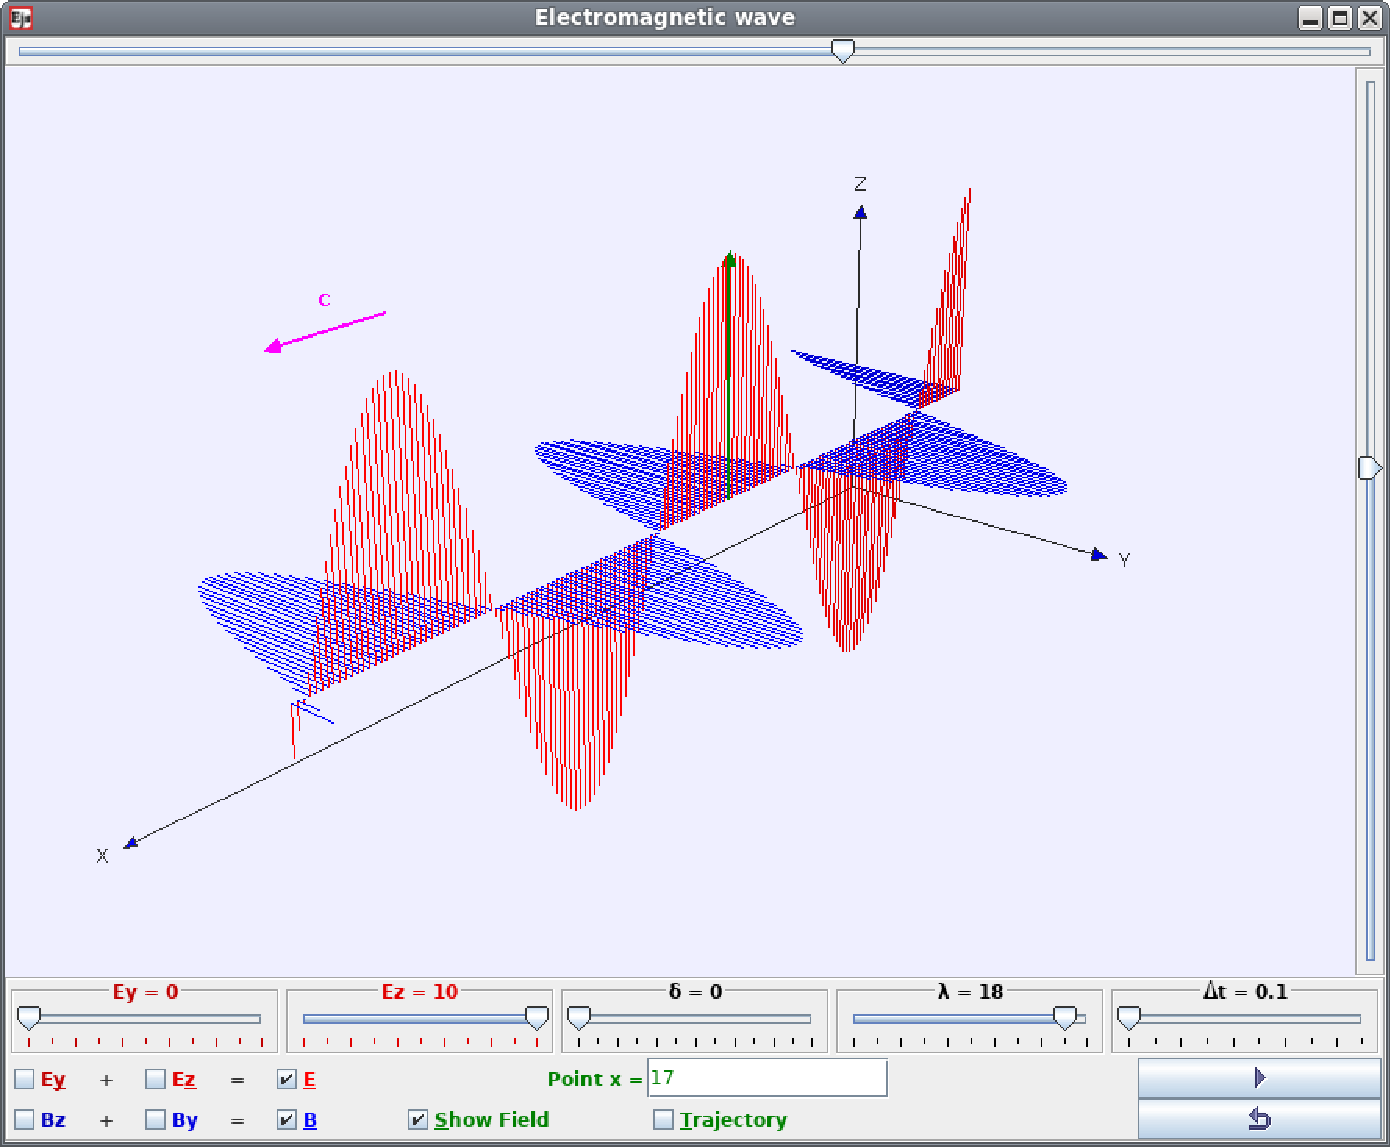
\includegraphics[height=5.50in]{plane_waves/planeWave1.pdf}
\caption{Java jar file showing plane electromagnetic waves.}
\index{color page}
\end{center}
\end{figure}

(f) The electromagnetic wave in this simulation is called a ``plane wave'' because its 
wavefronts are shaped like planes.  
What is the orientation of these planes?  
(Perpendicular to $\vec {E}$?  Perpendicular to the $z$ axis? Something else?)
\answerspace{20mm}
\end{comment}

\pagebreak[2]


\textbf{Activity 4: A Pencil-and-Paper Example Problem}

An electromagnetic \textbf{PLANE} wave is described by
\begin{align*}
\vv {E} &= E_{MAX} \cos \left ( kz - \omega t \right ) \hat x\\
\vv {B} &= B_{MAX} \cos \left ( kz - \omega t \right ) \hat y,
\end{align*}
and has a wavelength of $\lambda =12$ meters.  All $(x,y,z)$ points in this activity are in meters.
%\vspace{0.1in}

\begin{enumerate}[labparts]
\item Draw a sketch of the wave on the axes below, at time $t=0$.
%\begin{center}
%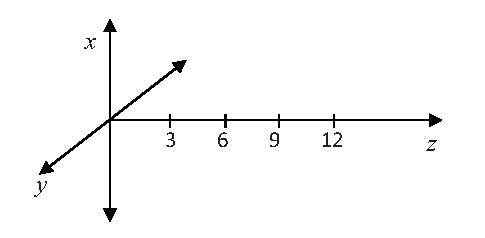
\includegraphics[width=0.4\textwidth]{plane_waves/em_waves_axes.eps}
%\end{center}

\begin{lab_axis}*[lab_noticks_3axes,
	width={3.0in}, height={1.8in},
	xmin=-1,xmax =15,
	xlabel={$z$~~~~~~~~~},  %a bit of a kludge to make "z" closer to the axis.
	ylabel=$y$,
	zlabel=$x$,
	xtick={3,6,9,12},
	]
\end{lab_axis}
\answerspace{0.1in}

\item At $t=0$, find both $\vv {E}$ and $\vv {B}$ at the points $(0,0,0), \,(0,0,3), \,(0,0,6),$ and $(0,0,9)$.  (Your answers are vectors, and should include both \textbf{magnitude} and \textbf{direction}.)  Your answers will be in terms of
$E_{MAX}$ and $B_{MAX}$.
\vspace{1.0in}

\item At $t=0$, find both $\vv {E}$ and $\vv {B}$ at the points $(0,1,0), \,(1,0,0), \,(1,1,0)$, and $(1,1,3)$.  (Remember, it's a \textbf{PLANE} wave….)
\vspace{1.0in}

\item Find the period $T$ and frequency $f$ of the wave.  (Numerical answers, please.)
\vspace{1.0in}

\item At $t=10$ nsec, find $\vv {E}$ and $\vv {B}$ at the points $(0,0,0), \,(0,0,3), \,(0,0,6), \,(0,0,9),$ and $(1,2,3)$.  
\vspace{1.0in}
\end{enumerate}


